\chapter{Object detection and segmentation}
In this thesis we focus on tracking objects in video data. Thus, we need to have a sensor for detecting objects in a
frame. Object detection is a fundamental task in computer vision that involves identifying and localizing objects
within images or video frames, respectively. Unlike image classification, which assigns a single label to an entire
image, object
detection algorithms aim to detect multiple objects of various classes and localize them with bounding boxes.

The development of object detection algorithms has evolved significantly over the years, driven by advances in deep
learning, dataset availability and computational power. Traditional object detection methods relied on handcrafted
features and machine learning algorithms, such as sliding window-based classifiers, histogram of oriented gradients (HOG), and Haar cascades. While effective in certain scenarios, these methods often lacked robustness and scalability, particularly in complex and cluttered scenes.

With the advent of deep learning, convolutional neural networks (CNNs) improved the field of object detection. CNNs are
capable of automatically learning hierarchical representations of data, making them well suited for image analysis
tasks. The rise of CNN-based approaches has led to significant improvements in object detection accuracy and efficiency.

Object detection poses several challenges, including variations in object appearance, scale, orientation, occlusion, and cluttered backgrounds. Additionally, real-world images often contain multiple objects of different classes, making it essential for detection algorithms to handle overlapping and partially visible objects.

Furthermore, object detection systems often have to balance accuracy and speed to meet the demands of real-time
applications. Achieving high detection accuracy while maintaining fast inference times is a fundamental challenge,
especially for devices with low hardware resources and applications requiring low-latency processing.

Object detection algorithms typically consist of several components:

\begin{itemize}
  \item \textbf{Input processing:} Images or video frames are preprocessed to standardize their format and size, often
involving resizing, normalization, and data augmentation to enhance model generalization.
  \item \textbf{Feature extraction:} Feature extraction is performed to capture relevant information from the input
  data. In deep learning-based approaches, convolutional neural networks (CNNs) are commonly used to extract hierarchical features that encode object appearance and spatial relationships.
  \item \textbf{Localization:} Localization involves predicting the spatial extent of objects within the image using
bounding boxes. This step requires regression or classification to estimate bounding box coordinates and confidence scores for object presence.
  \item \textbf{Classification:} Object classification assigns class labels to detected objects based on their visual
  appearance. Classification models are trained to distinguish between different object categories, enabling accurate identification of objects within the scene.
  \item \textbf{Post-processing:} Post-processing techniques, such as non-maximum suppression (NMS), are applied to
  refine detection results, suppress duplicate detections, and improve localization accuracy.
\end{itemize}

Object segmentation involves partitioning an image into semantically meaningful regions and associating each region
with a specific object instance. Unlike object detection, which identifies objects at the bounding box level, segmentation provides pixel-level delineation of object boundaries. This fine-grained information is invaluable for tasks such as image understanding, scene understanding and image manipulation.

Semantic segmentation assigns a class label to each pixel in the image, effectively partitioning the image into regions corresponding to different object categories. Fully Convolutional Networks (FCNs) and their variants, such as U-Net and DeepLab, have demonstrated remarkable success in semantic segmentation tasks by leveraging the power of convolutional neural networks for dense pixel-wise predictions.

Instance segmentation, on the other hand, extends semantic segmentation by distinguishing between individual object instances of the same class. This task requires not only segmenting objects but also differentiating between instances of the same class, even if they overlap or occlude each other. Mask R-CNN, an extension of Faster R-CNN, combines region-based object detection with instance segmentation, achieving state-of-the-art results in both tasks.

Despite significant advancements, object detection and segmentation still face several challenges. These include handling scale variations, occlusions, cluttered backgrounds, and fine-grained object attributes. Additionally, achieving real-time performance while maintaining high accuracy remains a critical goal for many applications.

\begin{figure}
  \centering
  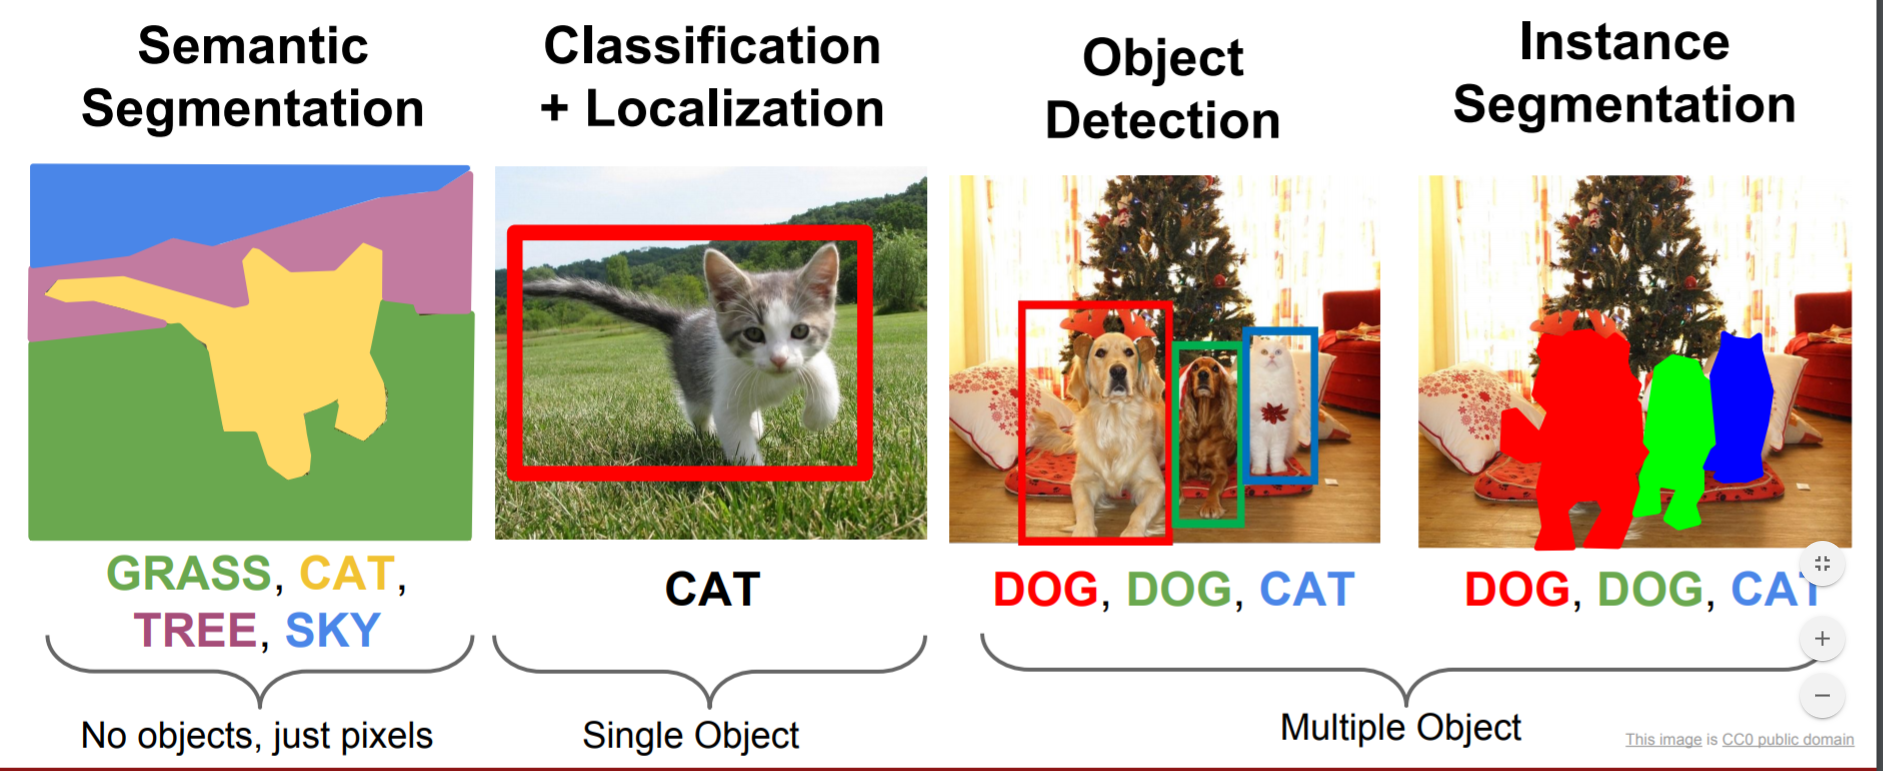
\includegraphics[width=\linewidth]{text/chapter_03/imgs/segmentation-types}
  \caption{Image detection and segmentation task types.}
  \label{fig:seg_type}
\end{figure}

\section{YOLO}
You Only Look Once (YOLO) is a revolutionary object detection algorithm that significantly transformed the field of computer vision. Developed by Joseph Redmon, Santosh Divvala, Ross Girshick, and Ali Farhadi, YOLO offers real-time object detection capabilities with impressive accuracy. This algorithm addresses the challenge of simultaneously detecting and classifying multiple objects within an image in a single forward pass through a convolutional neural network (CNN).

Traditionally, object detection systems involved multiple stages, including region proposal, feature extraction, classification, and post-processing. However, YOLO introduced a unified approach that directly predicts bounding boxes and class probabilities from the raw image data. This design not only simplifies the detection pipeline but also significantly accelerates inference speed, making it suitable for real-time applications.

At the core of YOLO is a single neural network that divides the input image into a grid and predicts bounding boxes and class probabilities for each grid cell. Each bounding box prediction includes coordinates (x, y) for the center of the box, width (w), height (h), and confidence score indicating the likelihood of containing an object. Additionally, class probabilities are estimated for each bounding box to determine the object category.

YOLO employs a loss function that penalizes localization errors, confidence errors, and classification errors. This loss function is optimized during training using labeled datasets to learn accurate object representations. Moreover, YOLO adopts anchor boxes to improve localization accuracy and handle scale variations of objects within the image.

One of the key advantages of YOLO is its impressive performance in terms of both accuracy and speed. By eliminating the need for multiple passes through the network and adopting a unified architecture, YOLO achieves state-of-the-art results while maintaining real-time processing capabilities. This makes it ideal for applications such as autonomous driving, surveillance systems, and robotics, where timely and accurate object detection is crucial.

However, YOLO also has its limitations. The fixed grid-based approach may struggle with detecting small objects or objects that are closely clustered together. Additionally, while YOLO is efficient for general object detection tasks, it may not perform as well as specialized algorithms in certain scenarios, such as detecting fine-grained object attributes or in highly cluttered environments.
\section{Segment Anything}